\subsubsection{Bayesian reweighting analysis}
\label{sec:projections:rw}

To quantify the impact of future
lattice QCD calculations on the NNPDF3.1 and NNPDFpol1.1
Monte Carlo sets (for the three scenarios of Tab.~\ref{tab:scenarios})
we use a procedure based on Bayesian reweighting analysis.
%
We briefly describe this procedure here,
and refer to~\cite{Ball:2011gg,Ball:2010gb} for
additional details.
\begin{itemize}
\item We first generate pseudo-data for the lattice-QCD calculations
 of $\la x\ra_{u^+}$,
$\la x\ra_{d^+}$,
$\la x\ra_{s^+}$,
$\la x\ra_{g}$, and
  $\la x\ra_{u^+-d^+}$ for the unpolarised case, and
  $\la 1\ra_{\Delta u^+}$,
$\la 1\ra_{\Delta d^+}$,
$\la 1\ra_{\Delta s^+}$,
$\la x\ra_{\Delta u^--\Delta d^-}$, and
  $\la 1\ra_{\Delta u^+ - \Delta d^+}$ for the polarised case.
  %
  We denote generically these moments by $\mathcal{F}_i$.
  
\item We construct the associated pseudo-data, denoted by $\mathcal{F}_i^{\rm (exp)}$,
  by taking the central values from
  the corresponding NNPDF fits, NNPDF3.1 NNLO for the unpolarised case and NNPDFpol1.1 NLO
  for the polarised one.
  %
  That is, we {\it assume} for simplicity that the central value
  of such future lattice calculations would coincide with the current ones
  from the global 
fit.\footnote{%
Repeating the exercise with the actual lattice QCD central values 
could be performed, but requires some choices as to how to impose 
the momentum sum rule, {c.f.}, Tab.~\ref{tab:BMunp}.
This  lies beyond the scope of the present studies.
}
  %
  As discussed in Sect.~\ref{sec:unpPDFs}, this corresponds to computing
  the mean over the Monte Carlo replica sample,
  \be
  \label{eq:pseudodatadef}
  \mathcal{F}_i^{\rm (exp)} \equiv \frac{1}{N_{\rm rep}}\sum_{k=1}^{N_{\rm rep}}
  \mathcal{F}_i^{\rm (k)} \, , \quad i=1,\ldots,N_{\rm mom} \, ,
  \ee
  where $N_{\rm mom}$ are the number of PDF moments that will be included
  in the reweighting, in this case $N_{\rm mom}=5$ both for the unpolarised
  and polarised cases.
  %
  To be consistent with the calculations in Sect.~\ref{sec:benchmarking},
  here the central values of the pseudo-data Eq.~(\ref{eq:pseudodatadef})
  are also evaluated at $Q^2=4$ GeV$^2$ (see Tabs.~\ref{tab:unpPDFmoms} and~\ref{tab:polPDFmoms}).
\item The uncertainty in the pseudo-data, denoted by $\delta\mathcal{F}_i^{\rm (exp)} $,
  is taken to be the value indicated in
  Tab.~\ref{tab:scenarios} for each of the three scenarios.
  %
  Thus, the absolute uncertainty on the $i$-th moment
  is given by $\delta\mathcal{F}_i^{\rm (exp)}=\delta_L^{(i)}\mathcal{F}_i^{\rm (exp)} $.
\item Using the pseudo-data (central values and total uncertainties)
  as defined above, we compute
  the Bayesian weights  $\omega_k$.
  %
  These weights
  quantify the agreement between each of $N_{\rm rep}$ replicas
  of the input PDF set and the corresponding lattice pseudo-data.
  %
  First of all, we compute the $\chi^2$ between each of the Monte Carlo
  replicas and the lattice pseudo-data as
  \be
  \chi^{2(k)}= \sum_{i=1}^{\rm N_{\rm mom}} \frac{\lp
    \mathcal{F}_i^{\rm (k)} -\mathcal{F}_i^{\rm (exp)} \rp^2}{
    \lp \delta\mathcal{F}_i^{\rm (exp)}\rp^2} \, , \quad k=1,\ldots,N_{\rm rep} \, ,
  \ee
  assuming that there are no correlations between the different $N_{\rm mom}$ moments.
  %
  This assumption in general might not be a good approximation, since most lattice
  QCD systematic errors are correlated among the different moments, and can be
  avoided, provided the full breakdown of systematic errors for each quantity is available.
  
  Once the values of the $\chi^2$ have been evaluated,
  we compute the corresponding weights for each replica.
  %
  The relation between the weights $w_k$  and the values of
  the $\chi^{2(k)}$ of each replica is
  \be
  \omega_k =\frac{\lp \chi^{2(k)} \rp^{(N_{\rm mom}-1)/2}\exp(-\chi^{2(k)}/2)}{
  \sum_{k=1}^{N_{\rm rep}} \lc \lp \chi^{2(k)} \rp^{(N_{\rm mom}-1)/2}\exp(-\chi^{2(k)}/2)\rc} \, ,
  \ee
  where the denominator ensures that the weight admit
  a probabilistic interpretation, that is, $\sum_k w_k=1$.
  %
  These weights represent a measure of the agreement of the individual replicas with the new pseudo-data.
  %
  For instance, replicas which have associated values
  of the moments far from the pseudo-data (within uncertainties) will
  have  a large $\chi^2$ and a very small weight, being thus effectively discarded.
\item These weights are used to recompute the PDFs, their moments,
  and generic cross-sections.
  %
  This procedure emulates the
  impact of adding lattice-QCD pseudo-data to a complete PDF fit.
  %
  For instance, after reweighting, the mean value of
  the PDF moments is
   \be
  \label{eq:pseudodatadef1}
  \mathcal{F}_i^{\rm (rw)} = \sum_{k=1}^{N_{\rm rep}}\omega_k
  \mathcal{F}_i^{\rm (k)} \, , \quad i=1,\ldots,N_{\rm mom} \, ,
  \ee
  with a similar relation for the associated uncertainties.
\end{itemize}

One limitation of this reweighting procedure is that it is only fully 
 reliable if the 
  effective number of replicas $N_{\rm eff}$ that survive the reweighting
  procedure (which is a measure of the amount
  of information left) is not too small.
  %
  This effective number of replicas
    is quantified in terms of the Shannon entropy
    \be
    \label{eq:effnrep}
    N_{\rm eff}\equiv \exp\lc \frac{1}{N_{\rm rep}}\sum_{k=1}^{N_{\rm rep}}\omega_k
    \log \lp N_{\rm rep}/\omega_k\rp\rc \, .
    \ee
    Finding that $N_{\rm eff}\ll N_{\rm rep}$ means that the pseudo-data
    has a large impact on the fit, potentially leading to a large
    reduction of the PDF uncertainties.
    %
    But if either the effective number of replicas becomes too
    small (say $N_{\rm eff}\lsim 25$), 
    or the relative fraction is small (say, $N_{\rm eff}/N_{\rm rep}\lsim 0.10$),
then the results
    become unreliable since they are affected by large
    statistical fluctuations.

    Therefore, before considering the effects
    of the lattice-QCD pseudo-data at the PDF
    level, we need to ensure that the
    three scenarios defined
    in Tab.~\ref{tab:scenarios} still lead
    to values of $N_{\rm eff}$ large enough for
    the reweighting procedure to be reliable.
  %
In Tab.~\ref{tab:neff} we indicate the effective number of replicas
    $N_{\rm eff}$, Eq.~(\ref{eq:effnrep}), remaining when the pseudo-data
    are included in the global
    fit according to the scenarios of Tab.~\ref{tab:scenarios}.
    %
    For completeness, we also indicate here the original number
    of replicas $N_{\rm rep}$ for the original
    PDF sets, NNPDF3.1   and NNPDFpol1.1 respectively.
    %
    As we can see, there is a marked decrease of $N_{\rm rep}$
    for the three scenarios, indicating that adding the
    PDF moments leads to non-trivial constraints on the global
    fit.
    %
    For instance, in the most optimistic scenario,
    scenario C, the effective number of replicas is around two (five) times
    smaller than the starting number of replicas in the unpolarised
    (polarised) case.

%%%%%%%%%%%%%%%%%%%%%%%%%%%%%%%%%%%%%%%%%%%%%%
% Moved these tables to the bottom of the page to follow the Appendix text
%
\begin{table}[h!]
  \centering
  \renewcommand{\arraystretch}{1.3} 
  \begin{tabular}{c|c|c}
    \hline
    &  NNPDF3.1  &  NNPDFpol1.1 \\
    \hline
    \hline
    $N_{\rm rep}$ original   &   1000 &  100   \\
    \hline
     $N_{\rm eff}$ Scenario A    &   740  &  72   \\
     $N_{\rm eff}$ Scenario B    &   750   &   59  \\
     $N_{\rm eff}$ Scenario C   &   510  &   20  \\
    \hline
  \end{tabular}
  \caption{\small The effective number of replicas
    $N_{\rm eff}$, Eq.~(\ref{eq:effnrep}), remaining when the pseudo-data
    on the PDF moments is included in the global
    fit according to the scenarios outlined
    in Tab.~\ref{tab:scenarios}.
    %
    For completeness, we also indicate the original number
    of replicas $N_{\rm rep}$ for the original
    PDF sets, NNPDF3.1   and NNPDFpol1.1 respectively.
    \label{tab:neff}
  }
\end{table}
%%%%%%%%%%%%%%%%%%%%%%%%%%%%%%%%%%%%%%%%%%%%%%

\paragraph{Impact on unpolarised global fits}
\label{subsec:upolfits}
%
We now discuss the results of applying the reweighting procedure
to a representative unpolarised
global fit, in this case the NNPDF3.1 analysis.
%
To begin with, in Tab.~\ref{tab:unpolmomentsrw} we summarise
the values of the unpolarised PDF moments
used as pseudo-data $\mathcal{F}_i^{(\rm exp)}$,
as well as the corresponding results
  after the reweighting has been performed, for the
three scenarios summarised 
in Tab.~\ref{tab:scenarios}.
%
The PDF uncertainties quoted there correspond to 68\%-CL intervals.
%
We recall that, as explained above, the three scenarios exhibit
uncertainties $\delta_L^{(i)}$ for the lattice-QCD pseudo-data rather smaller
than those of current state-of-the-art
calculations (see Tab.~\ref{tab:BMunp}).

%%%%%%%%%%%%%%%%%%%%%%%%%%%%%%%%%%%%%%%%%%%%%%%%%%%%%%%%
\begin{table}[t]
  \centering
  \renewcommand{\arraystretch}{1.4} 
\begin{tabular}{c||c|c|c|c}
  \hline &  Original  & Scen A  &  Scen B  &  Scen C  \\
  \hline
  \hline
  $\la x\ra_{u^+}$     &   $0.348 \pm  0.005$    &  $ 0.349 \pm 0.004$     &
  $ 0.349 \pm 0.004$   &  $ 0.349 \pm 0.003$   \\
  $\la x\ra_{d^+}$     &   $0.196\pm  0.004$     & $0.196 \pm0.004$       &
  $0.196 \pm0.003$ &   $0.196 \pm0.002$ \\
  $\la x\ra_{s^+}$     &   $0.0393 \pm 0.0036$   &  $0.0389\pm 0.0030$   &
 $0.0389\pm 0.0024$   &   $0.0389\pm 0.0014$  \\
  $\la x\ra_{g}$       &   $0.4097\pm 0.0042$    &  $0.4097 \pm 0.0043$    &
   $0.4097 \pm 0.0040$  &    $0.4097 \pm 0.0029$  \\
  $\la x\ra_{u^+-d^+}$  &   $0.1522 \pm 0.0033$   &  $0.1521 \pm 0.0037$   &
   $0.1521 \pm 0.0035$ &    $0.1521 \pm 0.0029$ \\
  \hline
\end{tabular}
\caption{\small Values of the unpolarised PDF moments
  used as pseudo-data, as well as the corresponding results
  after the reweighting has been performed, for the
three scenarios summarised 
in Tab.~\ref{tab:scenarios}.
%
The PDF uncertainties quoted correspond in all cases to 68\%
CL intervals.
\label{tab:unpolmomentsrw}
}
\end{table}
%%%%%%%%%%%%%%%%%%%%%%%%%%%%%%%%%%%%%%%%%%%%%%%%%%%%%%%%

From Tab.~\ref{tab:unpolmomentsrw} we see that a significant
reduction in the uncertainties in the unpolarised PDF moments is challenging to achieve
unless we assume the most aggressive scenarios.
%
For instance, in scenario C, which is about the best precision that
can achieved from lattice-QCD in the near future, the PDF uncertainties of the second moments
(that is, the momentum fractions) for $u^+,d^+,s^+$ and $g$ decrease by around
30\% to 60\%.
%
The most marked decrease is for the strange momentum fraction, since this is the
one affected by the largest PDF errors to begin with.
%
In contrast, the non-singlet combination $\la x\ra_{u^+-d^+}$ is essentially
unchanged in all three scenarios.
%
Note that, in Tab.~\ref{tab:unpolmomentsrw}, the central values of the PDF 
moments are stable, because we assume that the central values of the 
pseudo-data correspond to those of the input PDFs. 
%
In a realistic situation, such as that summarised in 
Figs.~\ref{fig:Bmomsunp}-\ref{fig:Bmomspol}, 
this is not necessarily the case and one expects
that the central values of the PDFs will also vary upon reweighting.

%------------------------------------------------------
\begin{figure}[!t]
\centering
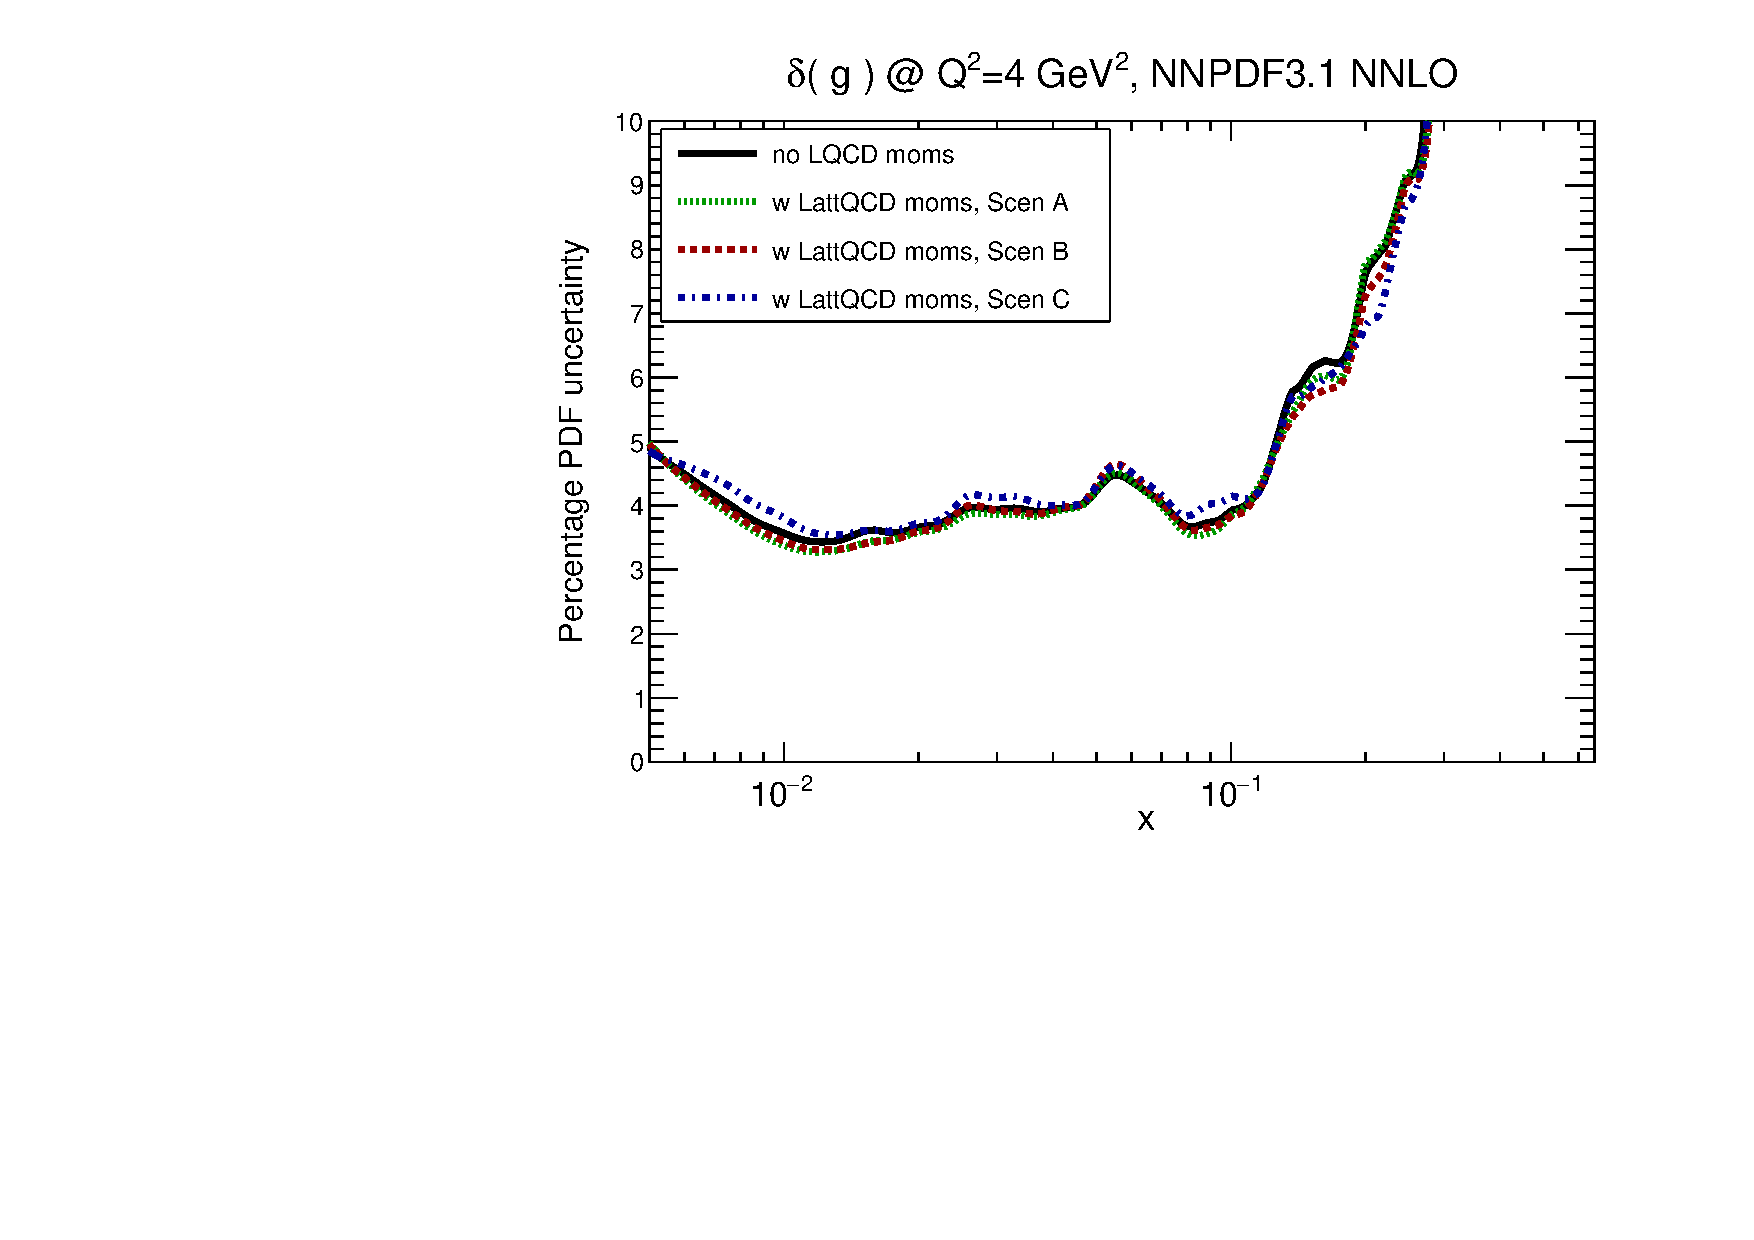
\includegraphics[scale=0.45]{plots/xg-unpol-lattice-relerr.pdf}
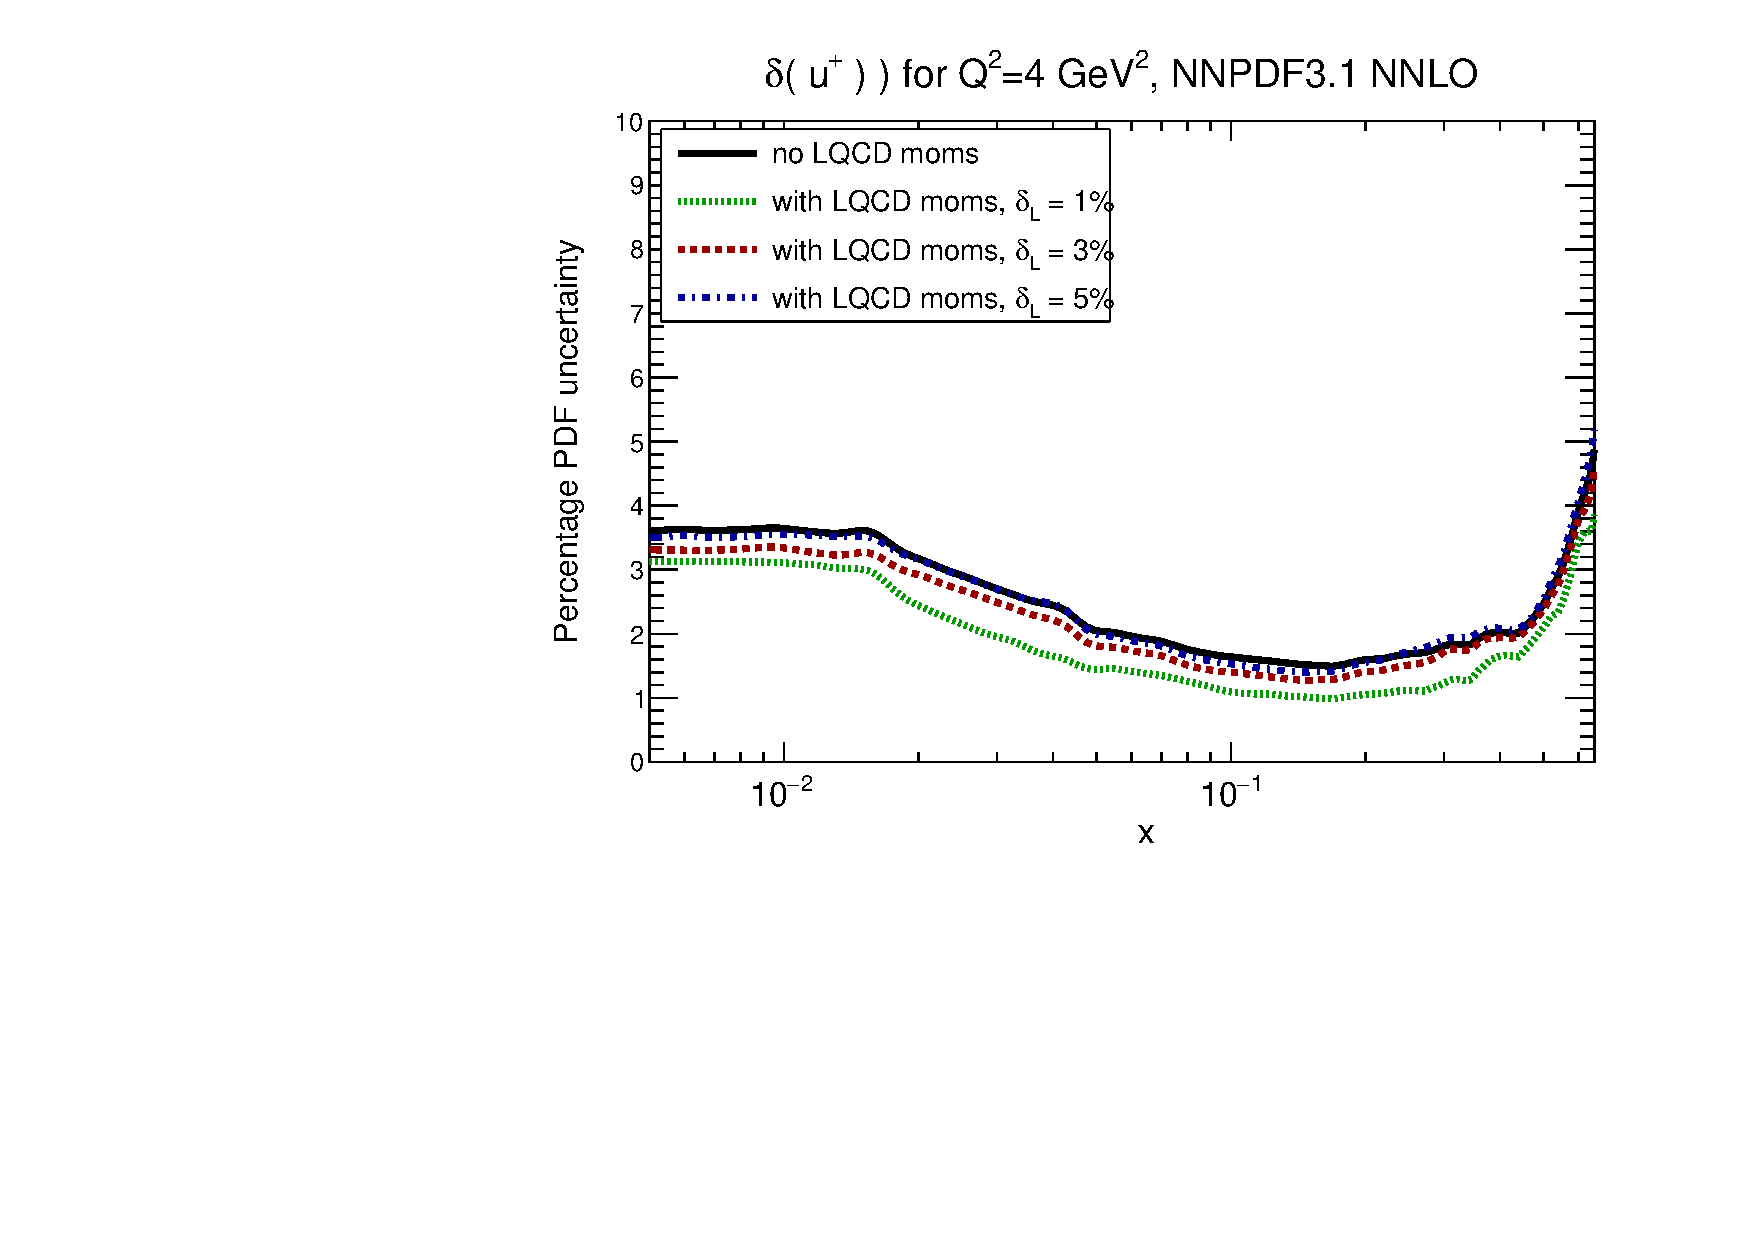
\includegraphics[scale=0.45]{plots/xup-unpol-lattice-relerr.pdf}
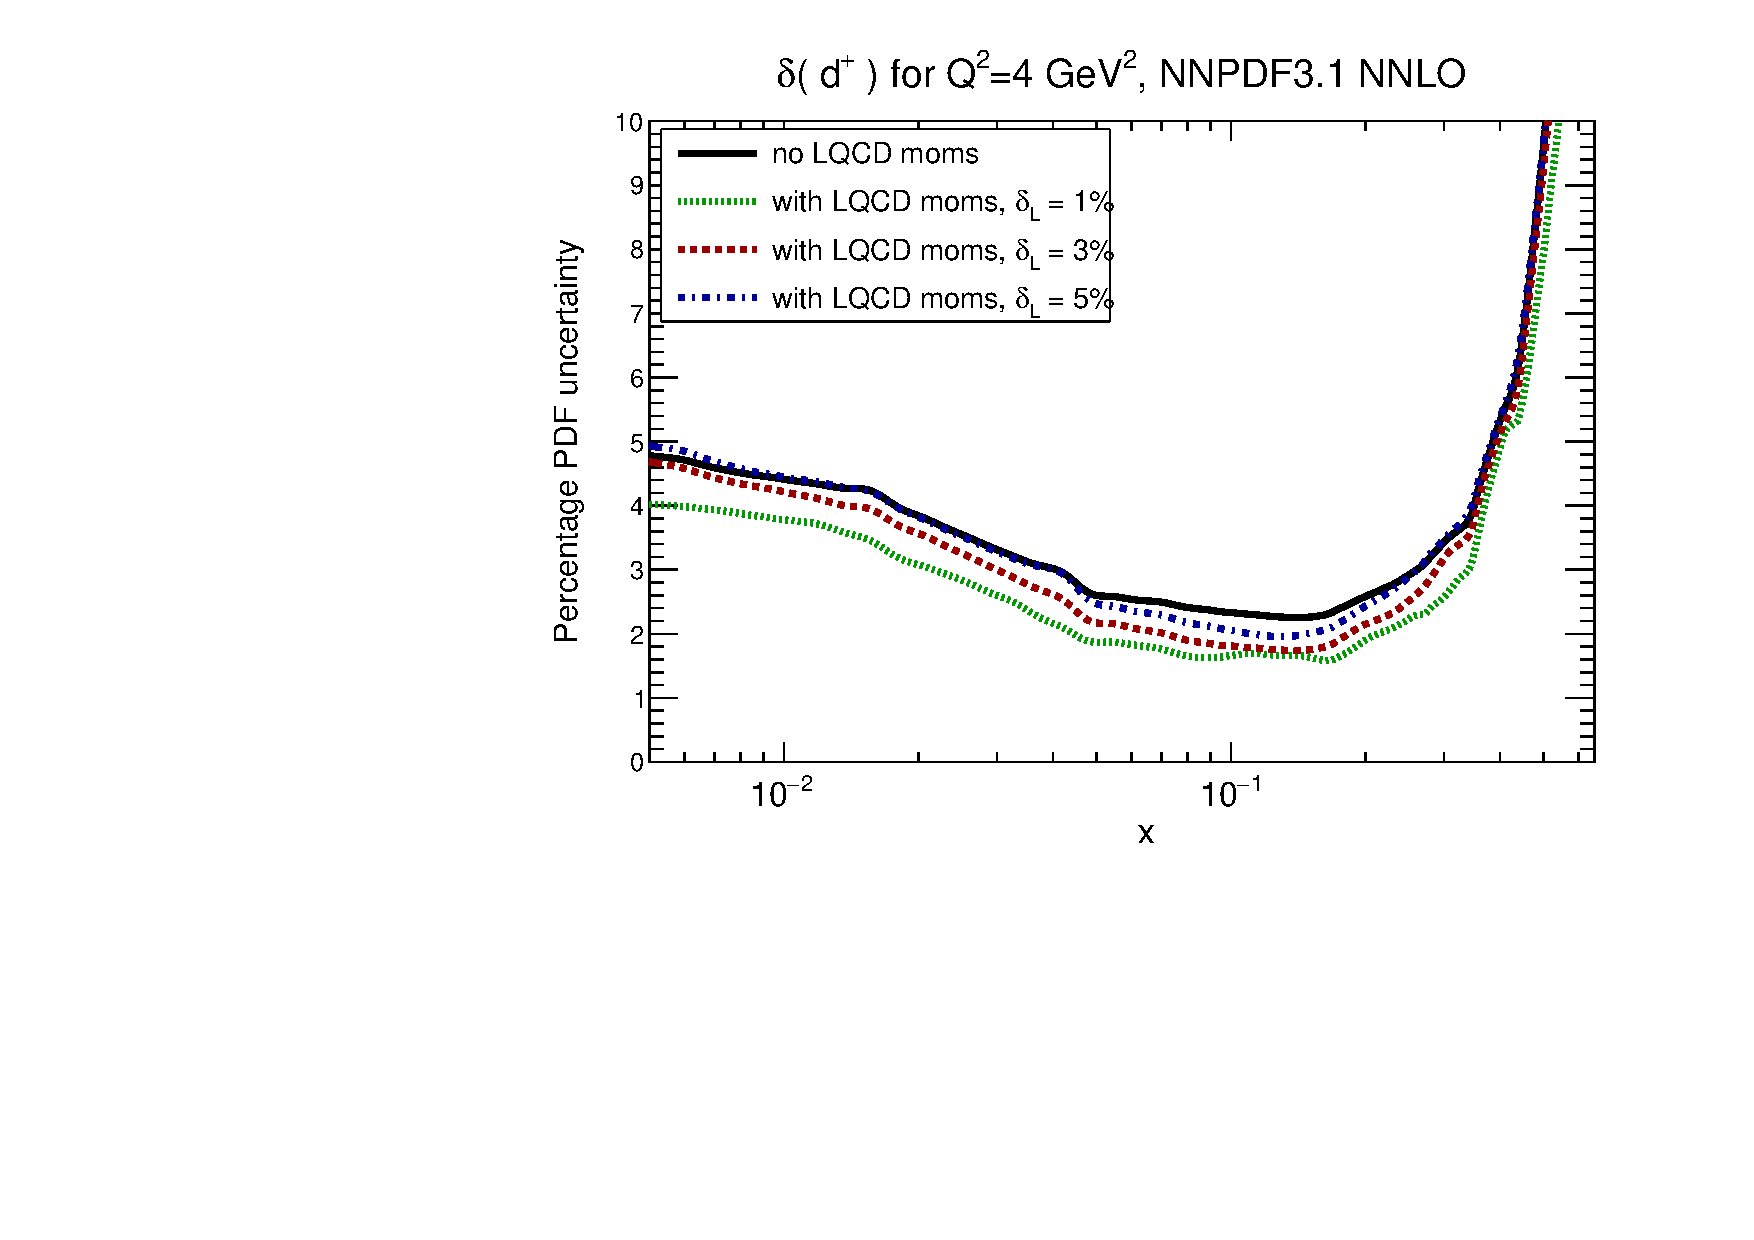
\includegraphics[scale=0.45]{plots/xdp-unpol-lattice-relerr.pdf}
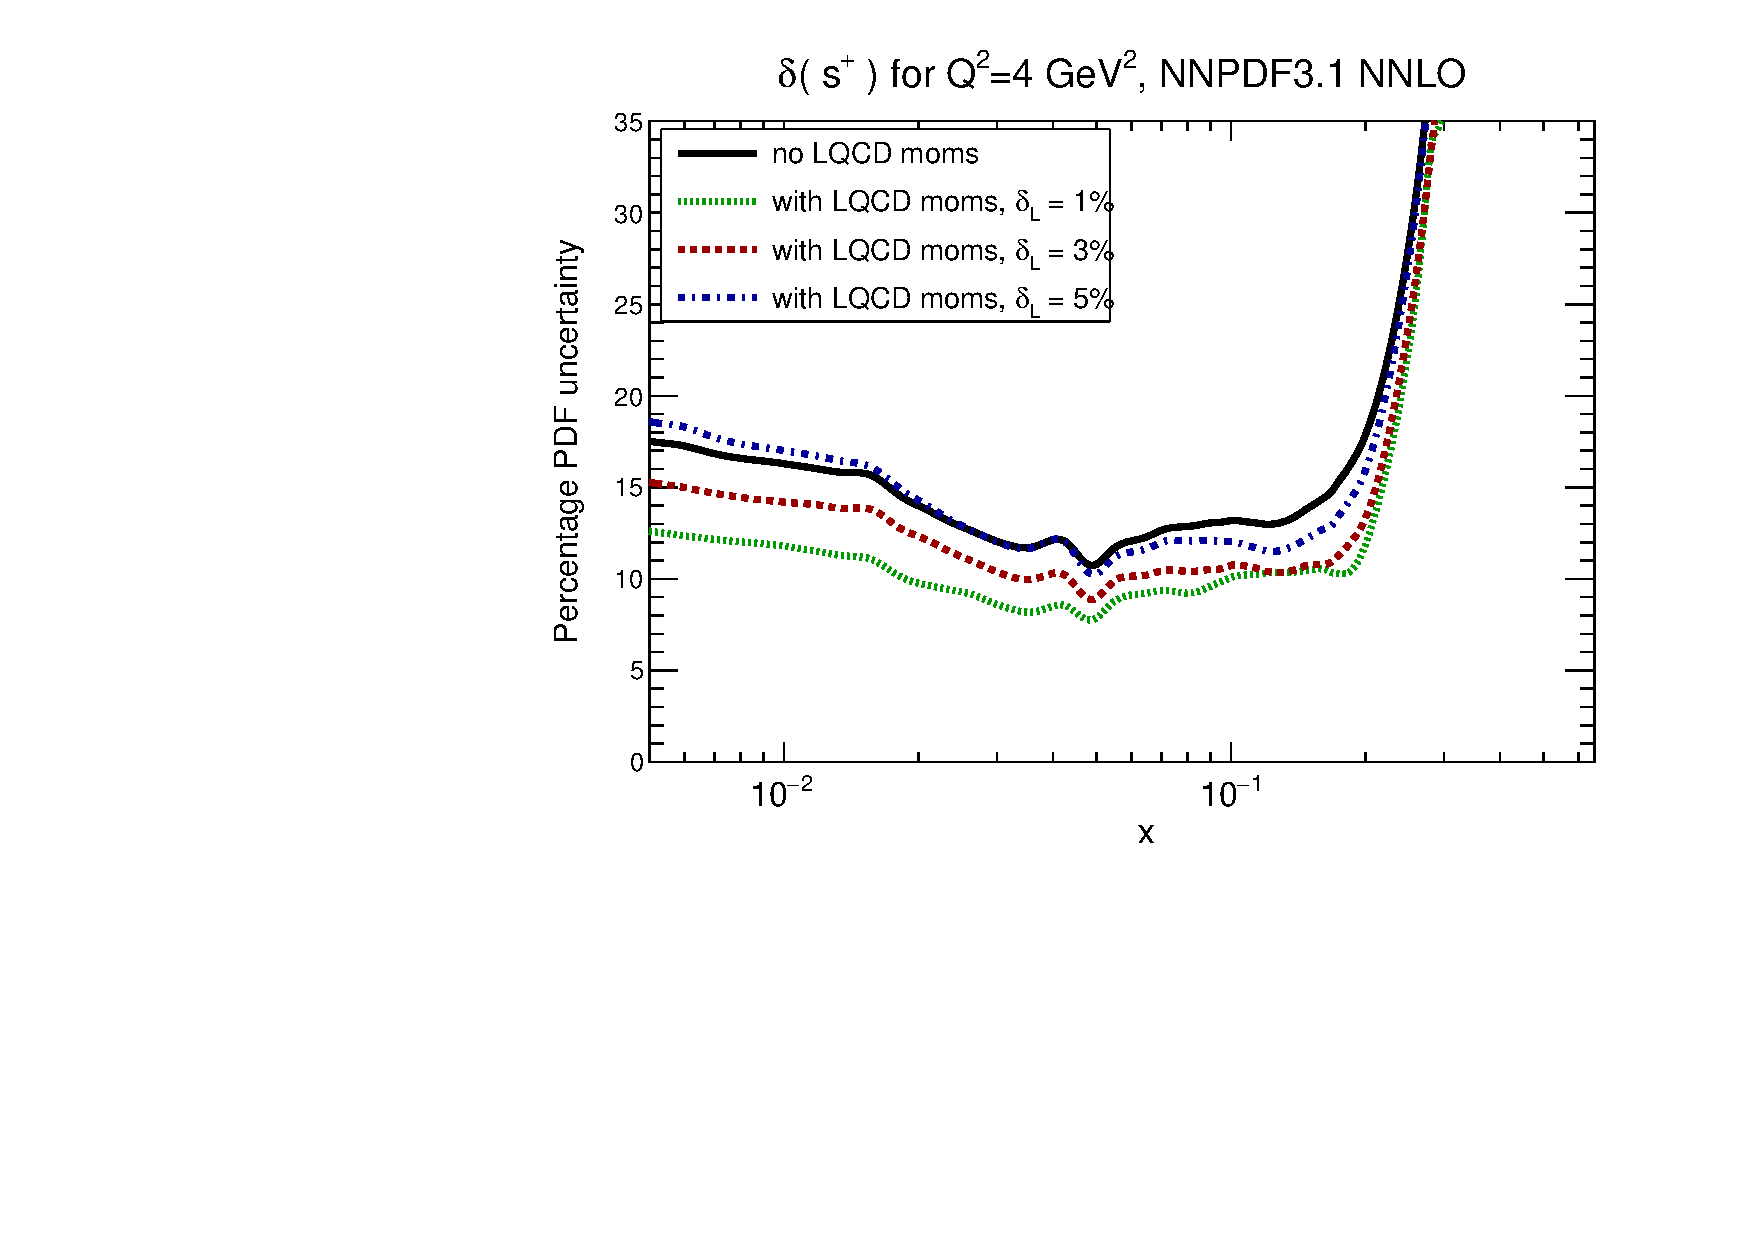
\includegraphics[scale=0.45]{plots/xsp-unpol-lattice-relerr.pdf}
\caption{\small The percentage PDF uncertainty in NNPDF3.1  
  for the gluon and the $u^+$, $d^+$ and $s^+$ quark PDFs at
  $Q^2=4$ GeV$^2$,
  compared to the results of including the five lattice
  QCD moments as pseudo-data points in the fit using the three
  different scenarios in  Tab.~\ref{tab:scenarios}.
  %
See text for more details.
}    
\label{fig:impactUnpol}
\end{figure}
%----------------------------------------------------------

Further evidence that reducing uncertainties in unpolarised PDFs will be 
challenging is shown in Fig.~\ref{fig:impactUnpol}, which plots the percentage 
PDF uncertainties in NNPDF3.1 for the gluon and the
$u^+$, $d^+$ and $s^+$ quark PDFs at $Q^2=4$ GeV$^2$, compared to the 
corresponding results including lattice-QCD pseudo-data.
%
In the case of the $u^+,d^+$ and $s^+$, we observe a slight reduction
of the PDF uncertainties, which is more marked as we move
from scenario A to C.
%
For instance, in the latter case the percentage PDF
uncertainty on $u^+$ ($d^+$ and $s^+$) at $x\simeq 0.1$
decreases from 1.8\% to 1.2\% (from 2.2\% to 1.7\% and from 13\% to 10\% respectively).
%
The PDF uncertainties of the gluon PDF, however,
are essentially unchanged even in the most optimistic scenario.

%%%%%%%%%%%%%%%%%%%%%%%%%%%%%%%%%%%%%%%%%%%
% 

We also observe the trend that the  reduction of the uncertainty 
of the PDF moments (cf.,  Tab.~\ref{tab:unpolmomentsrw})
is  more significant than the PDF uncertainty as a function of $x$  (Fig.~\ref{fig:impactUnpol}).
We will see this pattern also persists for the polarized PDF case
%
As the PDF moments integrate across all $x$  values (with emphasis at smaller $x$ values), 
this suggests there are correlation which could be driving this result.
%%%RST
In particular we note that in scenario C the uncertainty on the moment for 
$s^+$ is less than $4\%$ while for the PDF at any $x$ it is always greater 
than  $8\%$, a result which can only be acheived due to strong anticorrelation
between different $x$ regions. 
%%%% RST 
Additional studies examining the PDF correlations before and after inclusion of the 
QCD lattice could prove enlightening. 

%%%%%%%%%%%%%%%%%%%%%%%%%%%%%%%%%%%%%%%%%%%





Focusing on the large-$x$ region, where the
impact of the PDF moments considered here
is expected to be more marked, in
Fig.~\ref{fig:impactUnpollargex} we show a similar comparison
to that in Fig.~\ref{fig:impactUnpol}, but for the ratio 
of the uncertainties in each scenario as a ratio of the original PDF 
uncertainty of the NNPDF3.1 set, for the $d^+$
and $s^+$ total quark PDFs.
%
This comparison clearly illustrates that the relative reduction
of the PDF uncertainties upon the addition of the lattice-QCD
pseudo-data is not completely flat, and that it exhibits some
non-trivial structure.
%
We find that that the constraints from lattice-QCD calculations of these 
PDF moments is most pronounced for $x \simeq 0.2$, and decreases for larger 
values of $x$.

%------------------------------------------------------
\begin{figure}[!t]
\centering
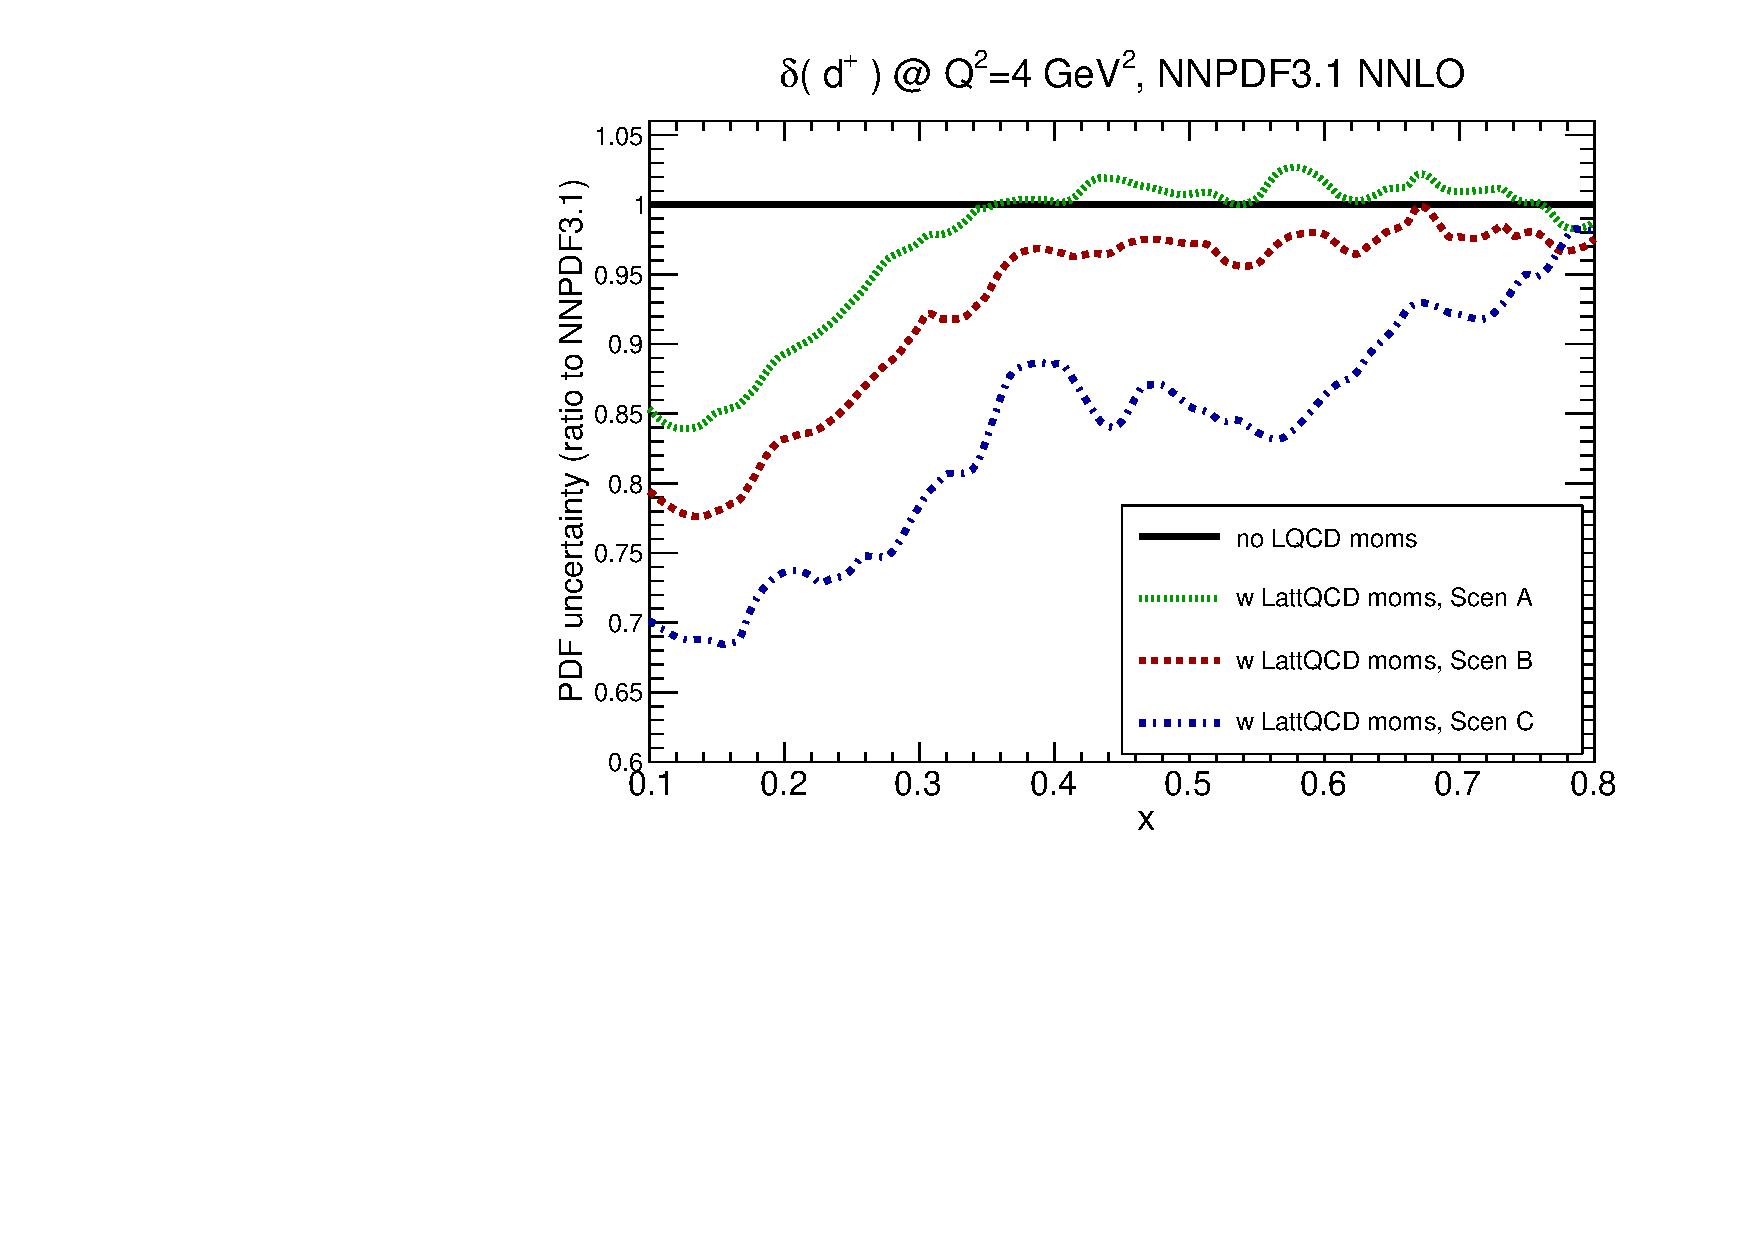
\includegraphics[scale=0.45]{plots/xdp-unpol-lattice-relerr-largex.pdf}
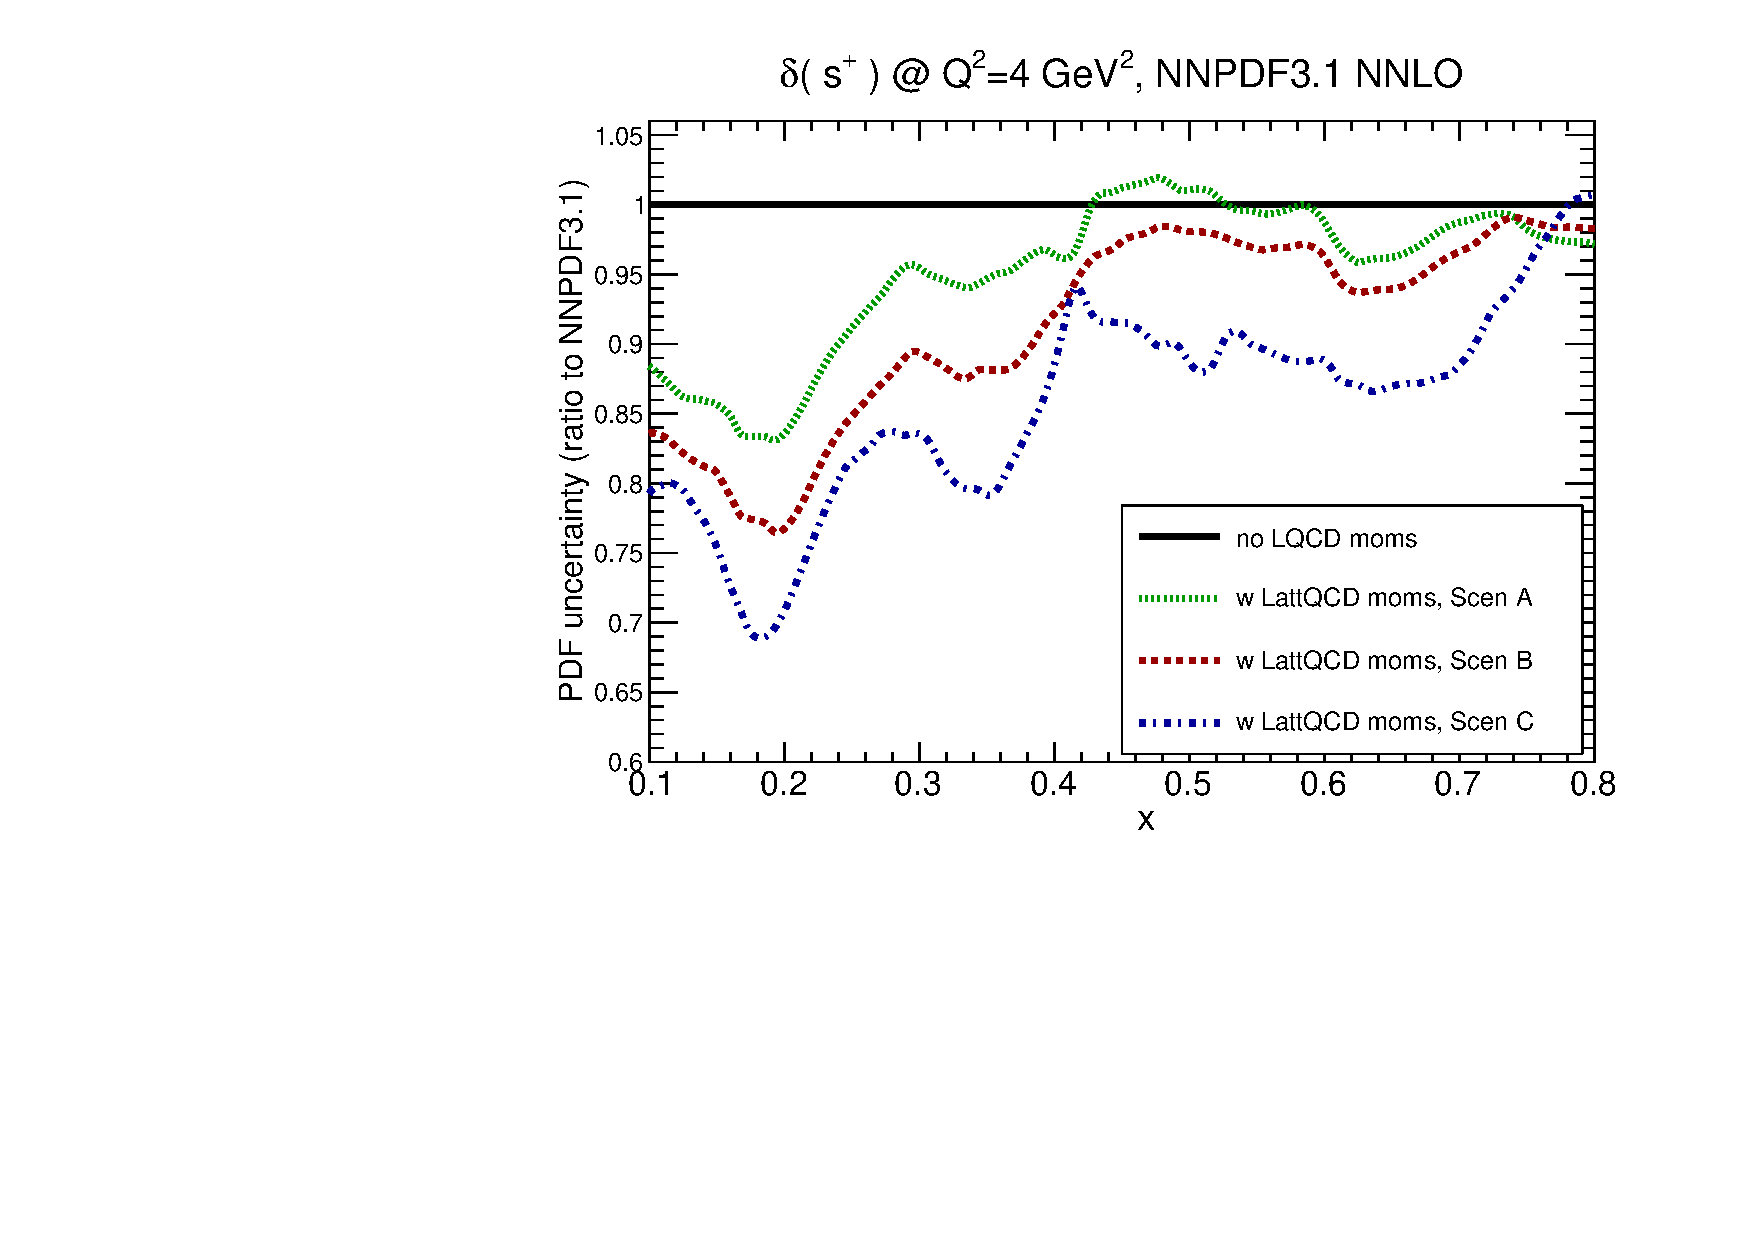
\includegraphics[scale=0.45]{plots/xsp-unpol-lattice-relerr-largex.pdf}
\caption{\small Same as Fig.~\ref{fig:impactUnpol}, now focusing
  on the large-$x$ region, and showing the ratio of the
  PDF uncertainties in the fits based on the three scenarios
  as a ratio of the original
  PDF uncertainty of the NNPDF3.1 set, for the $d^+$
  and $s^+$ total quark PDFs.
}    
\label{fig:impactUnpollargex}
\end{figure}
%----------------------------------------------------------

\paragraph{Impact on polarised global fits}
%
Now we turn to apply the
reweighting procedure to a representative polarised
global fit, the NNPDFpol1.1 NLO set.
%
In Tab.~\ref{tab:polmomentsrw}
we list the values of the polarised PDF moments
  used as pseudo-data, as well as the corresponding results
  after the reweighting has been performed for the
three scenarios summarised in 
in Tab.~\ref{tab:scenarios}.
%
As in the unpolarised case, the PDF uncertainties quoted correspond in all cases to 
68\%-CL intervals.
%
As we can see from this comparison, in scenario A
(which assumes lattice-QCD pseudo-data with similar uncertainties
to existing calculations) there is a marked impact on the
polarised PDF moments.
%
For both $\la 1\ra_{\Delta u^+}$ and $\la 1\ra_{\Delta d^+}$
the PDF uncertainties are roughly halved, with a similar, but less marked,
trend for $\la 1\ra_{\Delta s^+}$.
%
At this level, there is no impact on the non-singlet
combinations $\la 1\ra_{\Delta u^+ - \Delta d^+}$
and $\la x\ra_{\Delta u^--\Delta d^-}$.

%%%%%%%%%%%%%%%%%%%%%%%%%%%%%%%%%%%%%%%%%%%%%%%%%%%%%%%%
\begin{table}[t]
  \centering
  \renewcommand{\arraystretch}{1.4} 
\begin{tabular}{c||c||c|c|c}
  \hline &  Original  & Scen A  &  Scen B  & Scen C  \\
  \hline
  $\la 1\ra_{\Delta u^+}$    &  $+0.788\pm  0.079$   & $+0.798\pm  0.039$     &
  $+0.797\pm  0.023$ &   $+0.790\pm  0.009$ \\
  $\la 1\ra_{\Delta d^+}$   &  $-0.450 \pm 0.083$  &  $-0.450 \pm 0.042$  &
  $-0.456 \pm 0.026$    &  $-0.465 \pm 0.012$   \\
  $\la 1\ra_{\Delta s^+}$    &  $-0.124\pm   0.108 $  & $-0.120\pm   0.070 $  &
  $-0.121\pm   0.076 $    &   $-0.111\pm   0.029 $  \\
  $\la 1\ra_{\Delta u^+ - \Delta d^+}$  & $+1.250 \pm 0.024$   & $+1.250 \pm 0.022$  &
  $+1.253 \pm 0.016$ &    $+1.256 \pm 0.012$  \\
  $\la x\ra_{\Delta u^--\Delta d^-}$     & $+0.196 \pm 0.014$    & $+0.195 \pm 0.014$
  & $+0.196 \pm 0.016$     &  $+0.198 \pm 0.012$    \\
  \hline
\end{tabular}
\caption{\small Same as Tab.~\ref{tab:unpolmomentsrw}, now for
  the polarised PDF moments computed with NNPDFpol1.1.
  %
  The corresponding impact at the PDF level is shown in
  Fig.~\ref{fig:impactPol}.
\label{tab:polmomentsrw}
}
\end{table}
%%%%%%%%%%%%%%%%%%%%%%%%%%%%%%%%%%%%%%%%%%%%%%%%%%%%%%%%

As we further decrease the assumed uncertainties in the lattice-QCD
pseudo-data, we observe a corresponding reduction of the uncertainties
in the global fit.
%
In scenario C, the most optimistic, we find that for both
$\la 1\ra_{\Delta u^+}$ and $\la 1\ra_{\Delta d^+}$ there is an uncertainty
reduction by about an order of magnitude compared to the current values,
and about a factor of five for $\la 1\ra_{\Delta s^+}$.
%
Therefore, we demonstrate that future lattice-QCD calculations of
polarised PDF moments can potentially lead to a much more
precise understanding of the spin structure of the proton.
%
The other quark combinations exhibit less sensitivity to the inclusion
of the PDF moments in the global fit, because
they are already quite well constrained by available experimental
data.
%
The PDF uncertainties for  $\la 1\ra_{\Delta u^+ - \Delta d^+}$
are reduced by a factor of two in this quite optimistic scenario, while
those of $\la x\ra_{\Delta u^--\Delta d^-}$ are essentially unaffected even
in the most optimistic scenario.

%Next we move to illustrate the impact of the lattice-QCD pseudo-data
%on the polarised PDFs themselves, rather than on their
%moments.
%
%With this motivation,
In Fig.~\ref{fig:impactPol} we present a 
similar comparison to that of Fig.~\ref{fig:impactUnpol}, now
  showing the absolute PDF uncertainties of the NNPDFpol1.1 fit,
  compared to the corresponding results once the lattice pseudo-data
  on polarised moments is included in the analysis by means of the
  reweighting.
  %
  We show absolute rather than relative uncertainties
  because, unlike unpolarised PDFs, polarised PDFs often exhibit nodes
  (in particular for strangeness and the gluon) and in the nearby regions
  the concept of relative uncertainty becomes ill-defined.
  
%-------------------------------------------------------------------
\begin{figure}[!t]
\centering
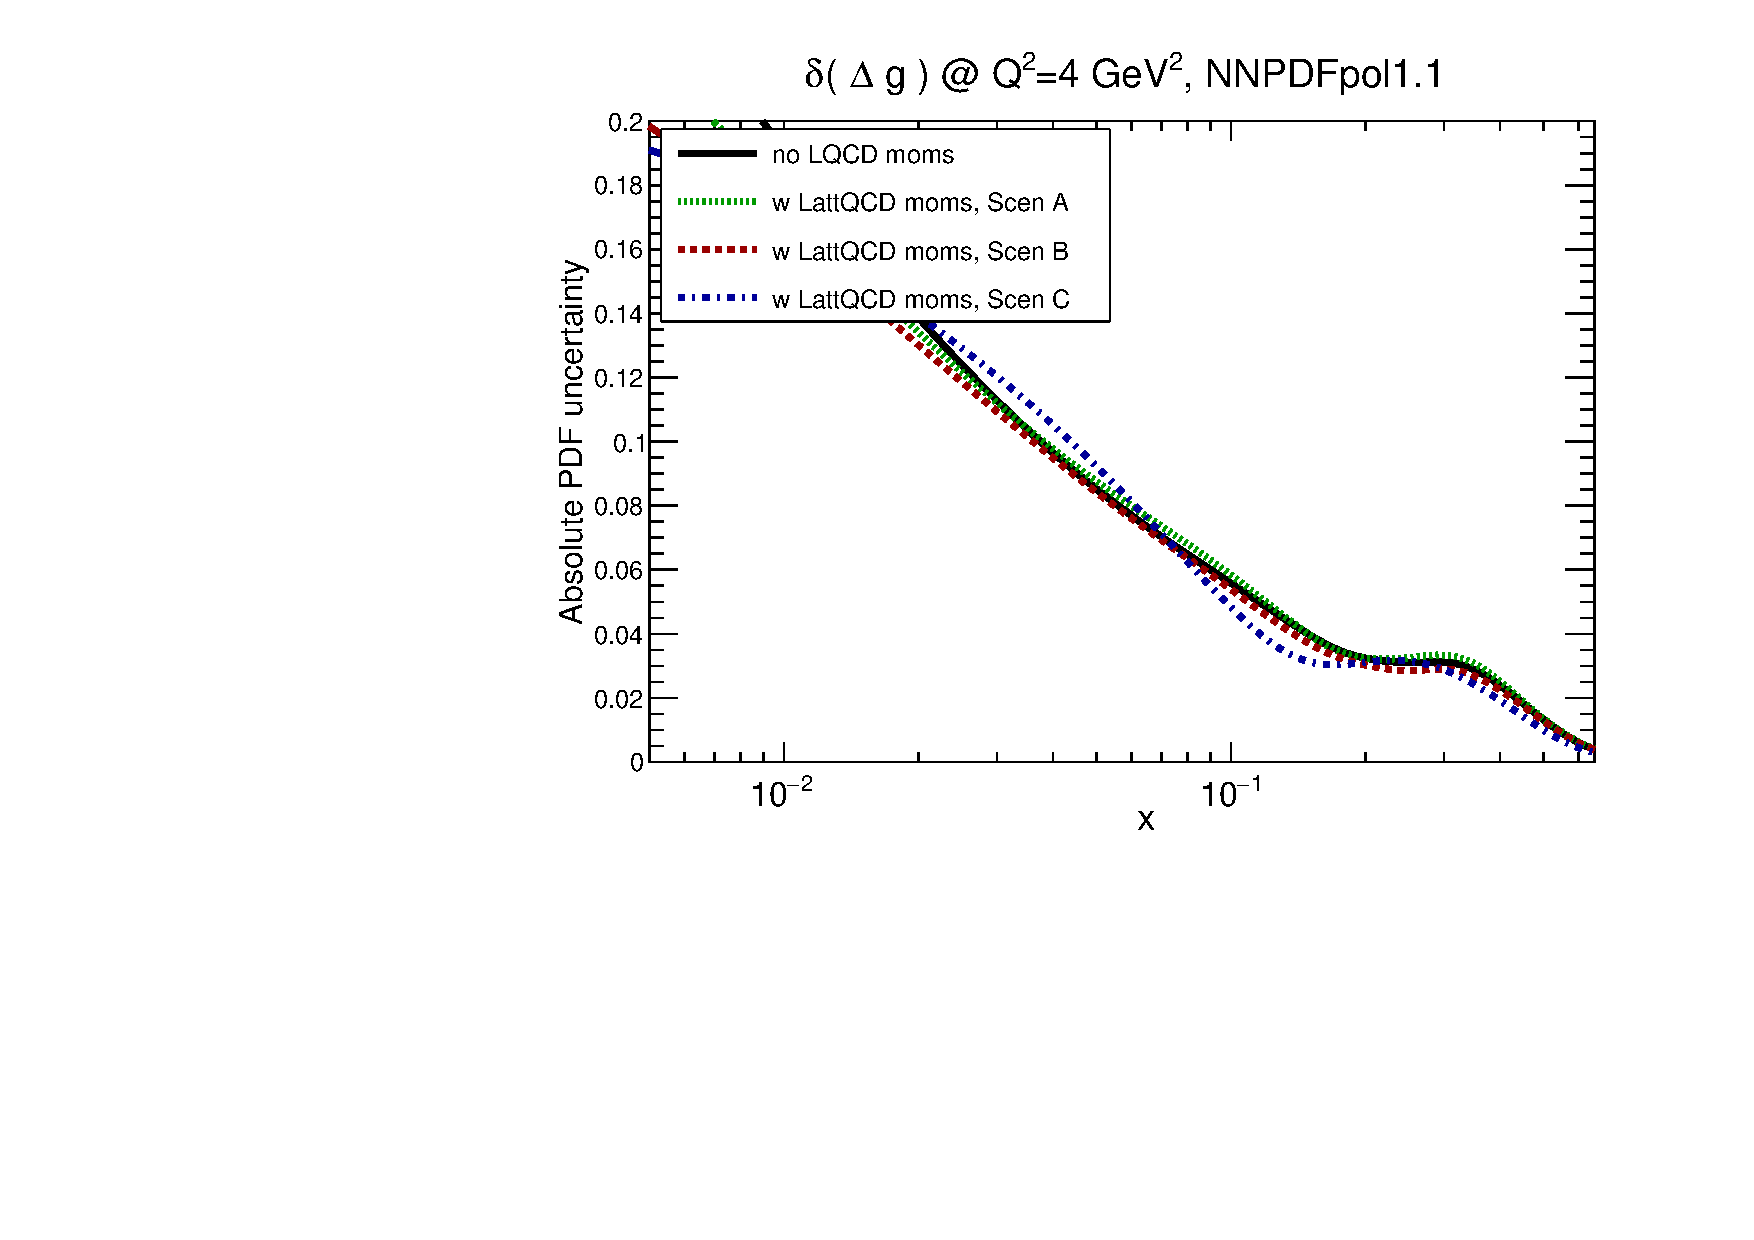
\includegraphics[scale=0.45]{plots/xg-pol-lattice-relerr.pdf}
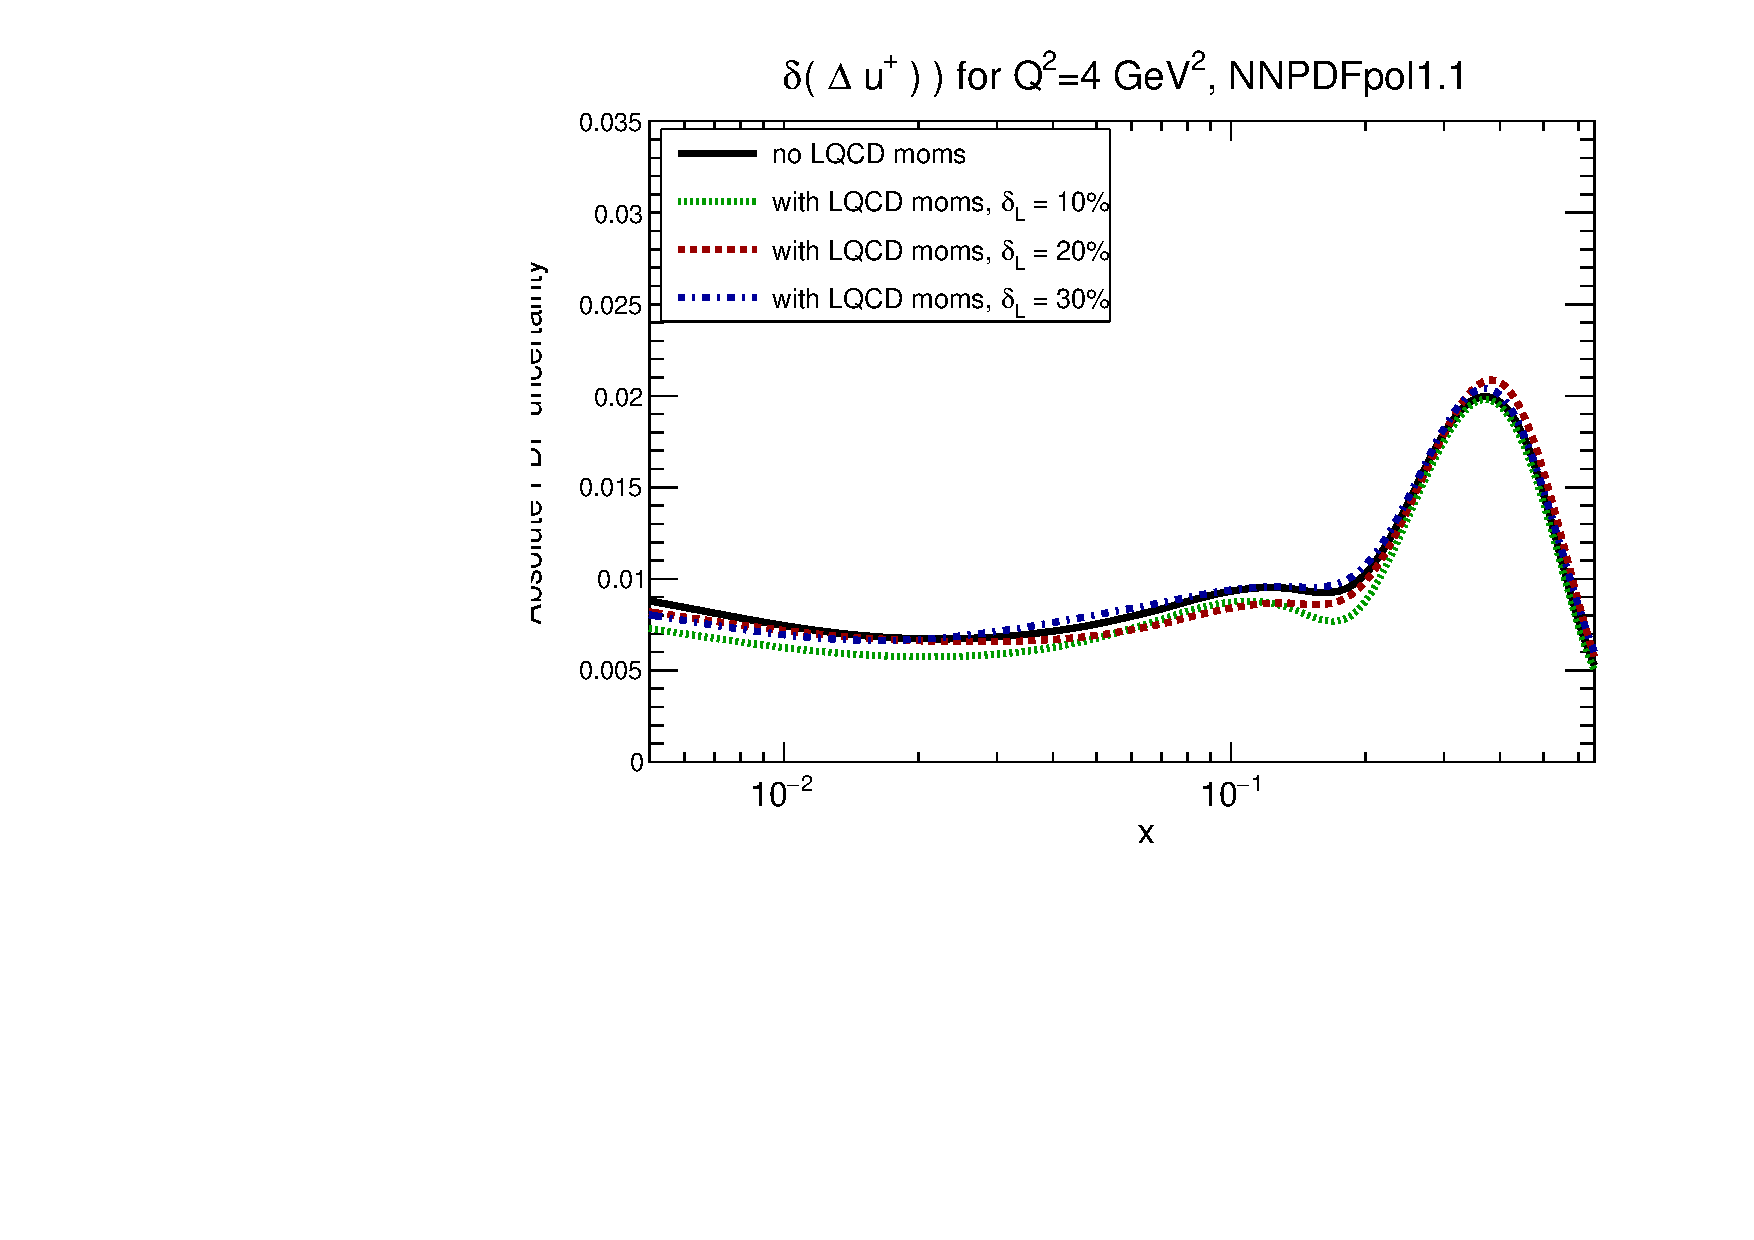
\includegraphics[scale=0.45]{plots/xup-pol-lattice-relerr.pdf}
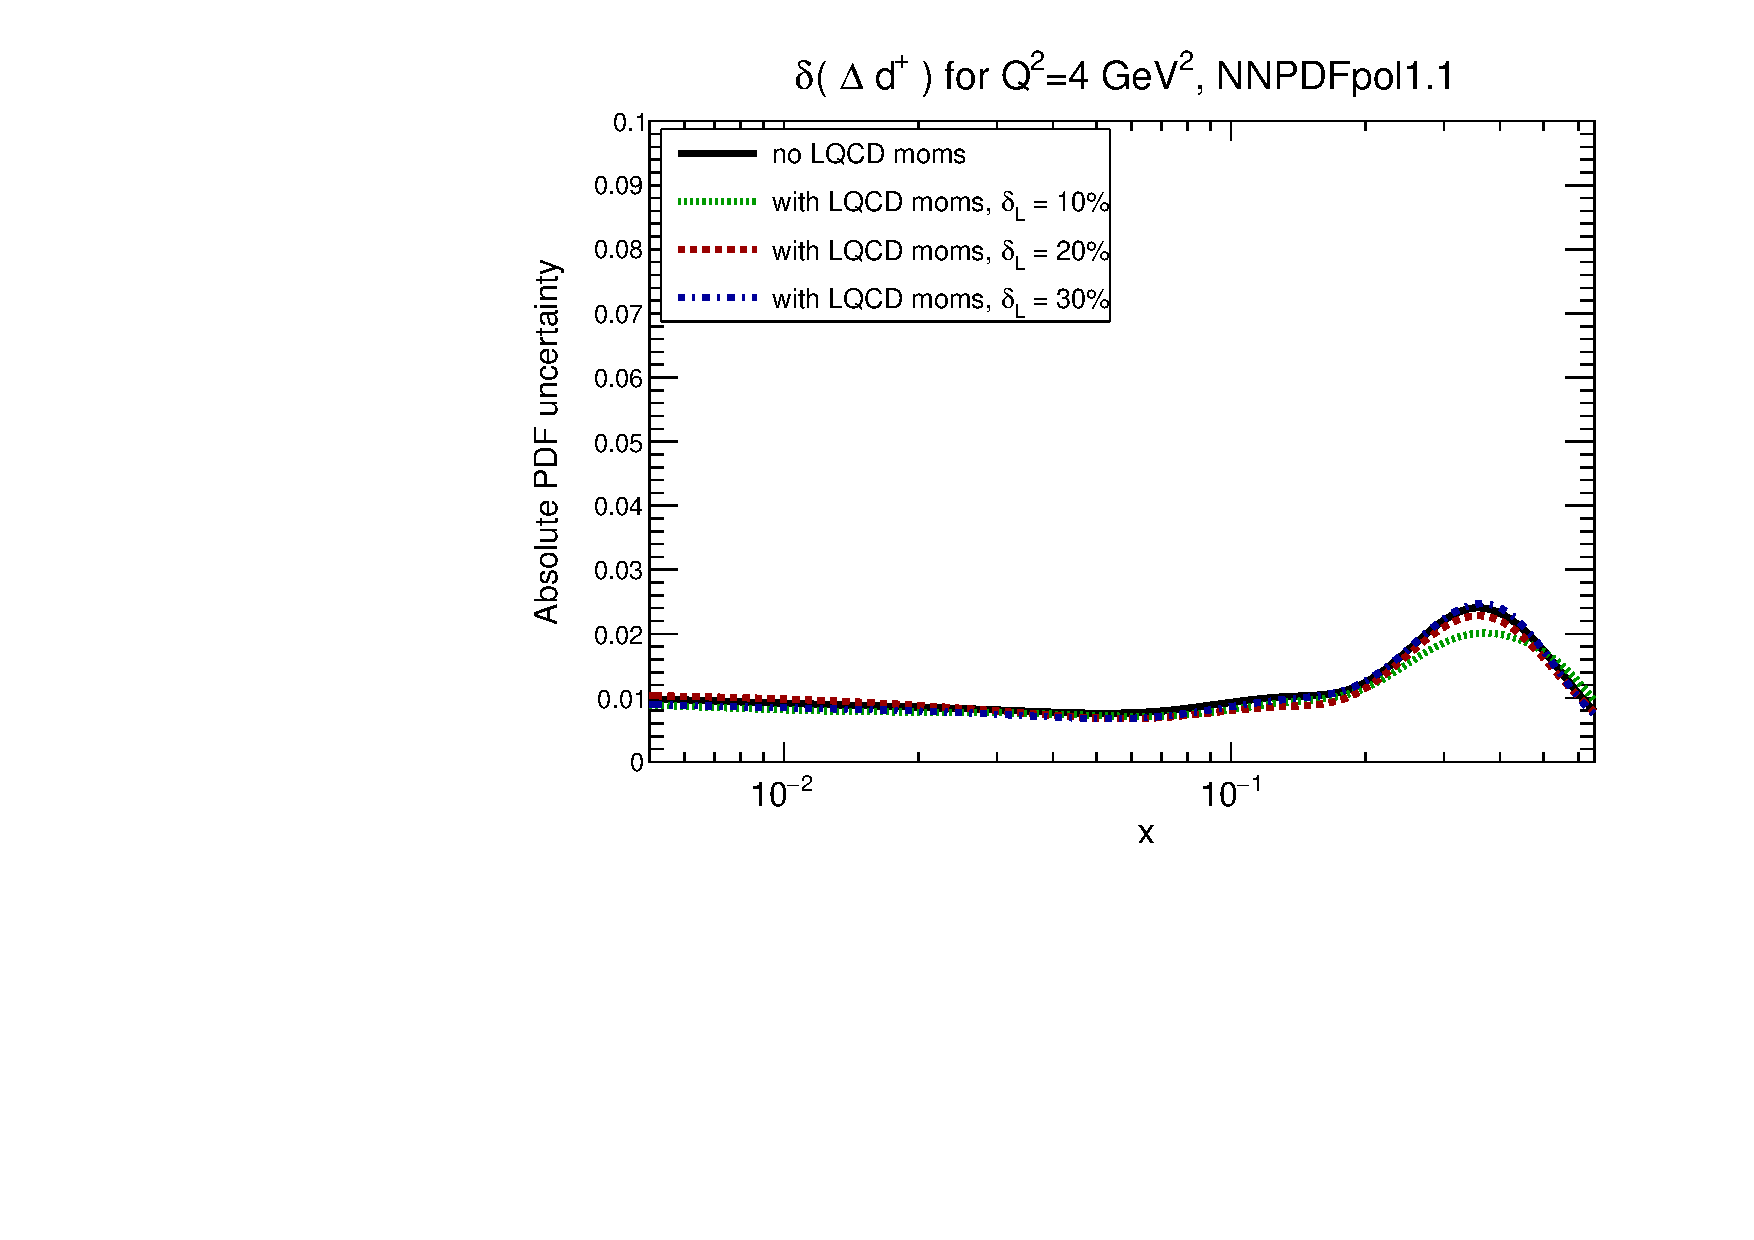
\includegraphics[scale=0.45]{plots/xdp-pol-lattice-relerr.pdf}
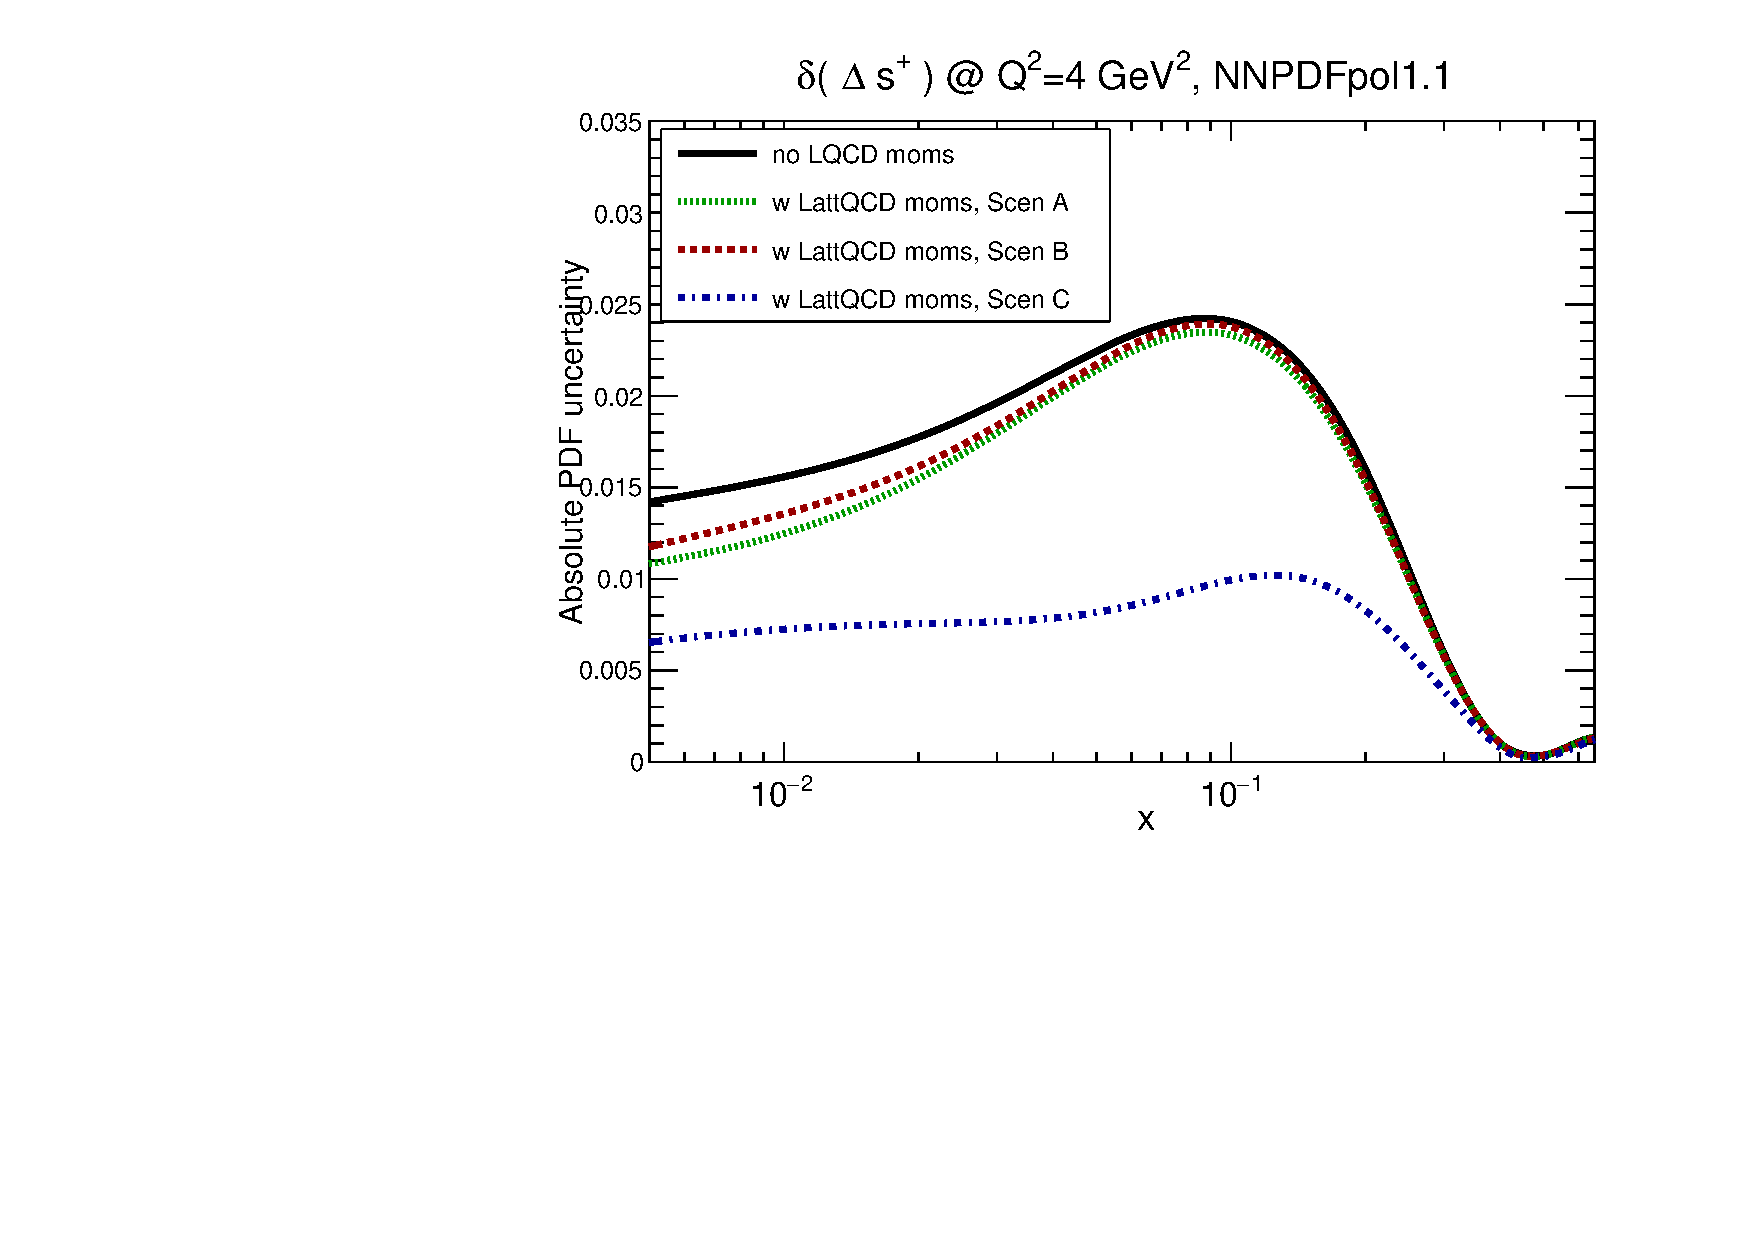
\includegraphics[scale=0.45]{plots/xsp-pol-lattice-relerr.pdf}
\caption{\small Same as Fig.~\ref{fig:impactUnpol}, now
  showing the absolute PDF uncertainties of the NNPDFpol1.1 fit
   $Q^2=4$ GeV$^2$,
  compared to the corresponding results once the lattice pseudo-data
  on polarised moments in included in the analysis via
  reweighting.
}    
\label{fig:impactPol}
\end{figure}
%---------------------------------------------------------------------

From Fig.~\ref{fig:impactPol} we see that for scenarios
A and B there is only a very moderate reduction (or even a slight increase)
of the PDF uncertainties, seemingly at odds with the results
for their moments in Tab.~\ref{tab:polmomentsrw}.
%
The reason is that the first PDF moments alone provide only limited
information on the shape of the PDFs themselves, and therefore in some
cases one finds a larger error reduction on the moments (since these
are the fitted quantities) than on the PDFs themselves (which are
only indirectly constrained).
%
Once, however, the lattice-QCD pseudo-data uncertainties
decrease beyond a certain level, these uncertainties start to influence the PDF shape, 
as we can see from the results of scenario C.
%
In that case we find that the PDF uncertainties can decrease by up to a factor
of two (three) for $\Delta d^+(x,Q)$ ($\Delta s^+(x,Q)$).
%%%%%RST
We also see the apparently simple feature that relative reduction of PDF uncertainties is more
or less constant along the whole range of $x$. 
%%%%% RST
For the strange quark this is perhaps 
roughly consistent with a simple reduction in the normalisation 
uncertainty indpendent of $x$.
However, similarly to the unpolarsied case, for the down quark this 
decrease is a much smaller 
factor than the decrease in the uncertainty of the moments, meaning that
there must be some anticorrelation between PDFs at different $x$ values.  
%%%%%RST

